\chapter{Electrical price}\label{sec:cost_fkt} %\todotom{I think it is a good idea to treat the data below as if it were a prediction of the future prices.
%W.r.t. the term 'cost function', I think it's a bit misplaced here. What you have in the graph is the cost-of-energy as a function of time. However, when you use the term 'cost function' it might be confused with the term 'objective function', which in your case will be the product between the cost-of-energy and the energy consumed.}
%
%
To minimize the running cost of the system, the power consumption of the pumps, $P_e$ Cf. \secref{PumpModel}, and the electrical price, $c_p[k]$, is considered. Predicting future prices is an extensive task that depends on many factors e.g user consumption and weather conditions. Due to the fact that the main focus of this project is not to derive a high precision predictive model that describe future electrical prices, data is used from \cite{Electrical_price} instead. The price function can be seen in \figref{fig:electrical_price}. 


% Due to the fact that the learning goals of this project is not to derive a high precision predictive model that describe future electrical prices, a simple model that mimics real electrical pricing is created. This model is based on electrical pricing in Denmark from the period 27-03-2017 to 02-04-2017.  


% To predict future prices a simple moving average (SMA) is used.
% This approach have been chosen, .

% The SMA uses present and previous data samples to calculate future predictions, this can be expressed as seen in \eqref{equ:MA}.
	
% \begin{equation}
% x(k+1) = \frac{1}{N}\sum\limits_{k=0}^{N-1} x(-k)
% \label{equ:MA}
% \end{equation} 

% The SMA can not take non-stationary processes into account, so if sudden changes in the price appears, the future estimates will be less precise. From \cite{Electrical_price} data price over the present has been gathered and can be seen on \figref{fig:electrical_price} together with the SMA model which utilize the previous data sample and the present. 

\begin{figure}[H]
\centering
% This file was created by matlab2tikz.
%
%The latest updates can be retrieved from
%  http://www.mathworks.com/matlabcentral/fileexchange/22022-matlab2tikz-matlab2tikz
%where you can also make suggestions and rate matlab2tikz.
%
\definecolor{mycolor1}{rgb}{0.00000,0.44700,0.74100}%
%
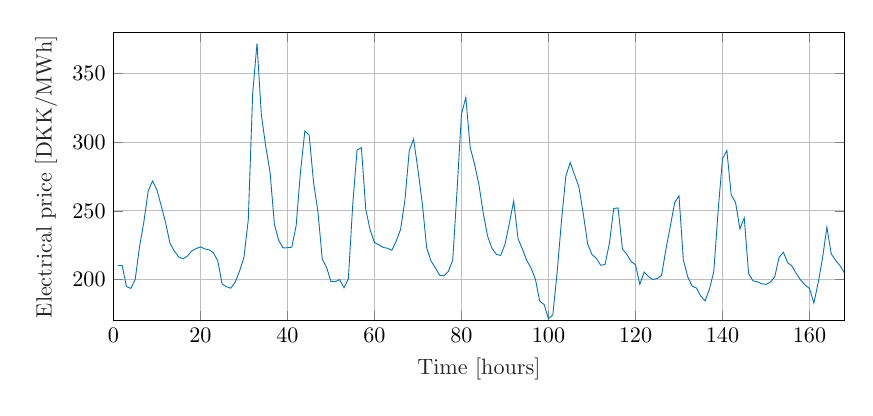
\begin{tikzpicture}[scale=0.8]

\begin{axis}[%
width=4.568in,
height=1.803in,
at={(0.766in,0.486in)},
scale only axis,
xmin=0,
xmax=168,
xlabel style={font=\color{white!15!black}},
xlabel={Time [hours]},
ymin=170,
ymax=380,
ylabel style={font=\color{white!15!black}},
ylabel={Electrical price [DKK/MWh]},
axis background/.style={fill=white},
xmajorgrids,
ymajorgrids
]
\addplot [color=mycolor1, forget plot]
  table[row sep=crcr]{%
1	210.15\\
2	210.3\\
3	194.9\\
4	193.565\\
5	200\\
6	223.91\\
7	242.07\\
8	264.61\\
9	271.82\\
10	265.2\\
11	253.6\\
12	241.32\\
13	226.44\\
14	220.72\\
15	216.55\\
16	215.14\\
17	217.07\\
18	220.86\\
19	222.5\\
20	223.84\\
21	222.35\\
22	221.68\\
23	219.52\\
24	213.425\\
25	196.72\\
26	194.745\\
27	193.74\\
28	198.17\\
29	206.24\\
30	216.21\\
31	243.7\\
32	335.1\\
33	372.01\\
34	320.15\\
35	297.16\\
36	278.26\\
37	240.24\\
38	228.49\\
39	223.05\\
40	223.2\\
41	223.58\\
42	239.27\\
43	278.71\\
44	308.09\\
45	305.12\\
46	270.82\\
47	249.69\\
48	215.02\\
49	208.76\\
50	198.72\\
51	198.49\\
52	200.06\\
53	194.1\\
54	200.5\\
55	254.14\\
56	294.32\\
57	295.96\\
58	251.24\\
59	236.29\\
60	227.06\\
61	225.35\\
62	223.42\\
63	222.82\\
64	221.33\\
65	228.03\\
66	236.44\\
67	257.71\\
68	293.87\\
69	302.28\\
70	279.89\\
71	255.33\\
72	223.12\\
73	213.55\\
74	208.49\\
75	203.13\\
76	202.76\\
77	206.03\\
78	214.36\\
79	265.7\\
80	320.39\\
81	332.67\\
82	296.21\\
83	284.155\\
84	269.35\\
85	248.555\\
86	231.7\\
87	222.77\\
88	218.455\\
89	217.565\\
90	225.6\\
91	240.815\\
92	257.22\\
93	229.88\\
94	222.25\\
95	213.99\\
96	208.41\\
97	200.18\\
98	184.26\\
99	181.88\\
100	171.47\\
101	174.44\\
102	205.58\\
103	243.22\\
104	275.54\\
105	285.25\\
106	276.175\\
107	267.28\\
108	247.87\\
109	226.035\\
110	218.22\\
111	215.435\\
112	210.45\\
113	210.97\\
114	226.37\\
115	251.74\\
116	252.18\\
117	222.2\\
118	218.56\\
119	213.2\\
120	210.82\\
121	196.56\\
122	205.48\\
123	202.14\\
124	200.06\\
125	200.8\\
126	203.1\\
127	222.14\\
128	238.65\\
129	255.98\\
130	261.04\\
131	214.26\\
132	202.14\\
133	195.26\\
134	193.88\\
135	188.08\\
136	184.51\\
137	193.1\\
138	205.82\\
139	250.33\\
140	287.81\\
141	294.06\\
142	261.71\\
143	256.2\\
144	236.94\\
145	244.83\\
146	204.52\\
147	199.09\\
148	198.35\\
149	197.01\\
150	196.49\\
151	198.2\\
152	201.85\\
153	216.13\\
154	219.84\\
155	212.26\\
156	209.73\\
157	204.15\\
158	199.47\\
159	196.04\\
160	193.52\\
161	182.88\\
162	197.72\\
163	215.825\\
164	238.21\\
165	218.65\\
166	214.04\\
167	210.18\\
168	204.97\\
};
\end{axis}
\end{tikzpicture}%
\caption{$c_p[k]$, describing the electricity prices in Denmark from the 27-03-2017 to 02-04-2017.}
\label{fig:electrical_price} 
\end{figure}

As this is a real data from a given period, most likely it does not fit the pricing in any other given week, as the pricing is fluctuating a lot from day to day. However, the data indicates that the pricing is higher in the morning and evening which is applicable for any given week and thereby is a general property of the time dependent pricing. This behavior can be seen as the periodicity of the data with two peaks a day. The chosen data thus gives a realistic idea of the improvement of the controller which can be achieved in a real world scenario based on the week on which the data is recorded.  

%However $\frac{1}{\eta}\cdot\Delta p \cdot q \cdot \Gamma(k)$ 

% Even though the pricing seen in \figref{fig:electrical_price} is not a prediction of the future electrical pricing it is assumed to be a good representation of the pricing and therefor it will be used for this project. 
